% Options for packages loaded elsewhere
\PassOptionsToPackage{unicode}{hyperref}
\PassOptionsToPackage{hyphens}{url}
%
\documentclass[
]{article}
\usepackage{amsmath,amssymb}
\usepackage{lmodern}
\usepackage{iftex}
\ifPDFTeX
  \usepackage[T1]{fontenc}
  \usepackage[utf8]{inputenc}
  \usepackage{textcomp} % provide euro and other symbols
\else % if luatex or xetex
  \usepackage{unicode-math}
  \defaultfontfeatures{Scale=MatchLowercase}
  \defaultfontfeatures[\rmfamily]{Ligatures=TeX,Scale=1}
\fi
% Use upquote if available, for straight quotes in verbatim environments
\IfFileExists{upquote.sty}{\usepackage{upquote}}{}
\IfFileExists{microtype.sty}{% use microtype if available
  \usepackage[]{microtype}
  \UseMicrotypeSet[protrusion]{basicmath} % disable protrusion for tt fonts
}{}
\makeatletter
\@ifundefined{KOMAClassName}{% if non-KOMA class
  \IfFileExists{parskip.sty}{%
    \usepackage{parskip}
  }{% else
    \setlength{\parindent}{0pt}
    \setlength{\parskip}{6pt plus 2pt minus 1pt}}
}{% if KOMA class
  \KOMAoptions{parskip=half}}
\makeatother
\usepackage{xcolor}
\usepackage[margin=1in]{geometry}
\usepackage{longtable,booktabs,array}
\usepackage{calc} % for calculating minipage widths
% Correct order of tables after \paragraph or \subparagraph
\usepackage{etoolbox}
\makeatletter
\patchcmd\longtable{\par}{\if@noskipsec\mbox{}\fi\par}{}{}
\makeatother
% Allow footnotes in longtable head/foot
\IfFileExists{footnotehyper.sty}{\usepackage{footnotehyper}}{\usepackage{footnote}}
\makesavenoteenv{longtable}
\usepackage{graphicx}
\makeatletter
\def\maxwidth{\ifdim\Gin@nat@width>\linewidth\linewidth\else\Gin@nat@width\fi}
\def\maxheight{\ifdim\Gin@nat@height>\textheight\textheight\else\Gin@nat@height\fi}
\makeatother
% Scale images if necessary, so that they will not overflow the page
% margins by default, and it is still possible to overwrite the defaults
% using explicit options in \includegraphics[width, height, ...]{}
\setkeys{Gin}{width=\maxwidth,height=\maxheight,keepaspectratio}
% Set default figure placement to htbp
\makeatletter
\def\fps@figure{htbp}
\makeatother
\setlength{\emergencystretch}{3em} % prevent overfull lines
\providecommand{\tightlist}{%
  \setlength{\itemsep}{0pt}\setlength{\parskip}{0pt}}
\setcounter{secnumdepth}{5}
\usepackage{booktabs}
\usepackage{amsthm}
\makeatletter
\def\thm@space@setup{%
  \thm@preskip=8pt plus 2pt minus 4pt
  \thm@postskip=\thm@preskip
}
\makeatother
\ifLuaTeX
  \usepackage{selnolig}  % disable illegal ligatures
\fi
\usepackage[]{natbib}
\bibliographystyle{plainnat}
\IfFileExists{bookmark.sty}{\usepackage{bookmark}}{\usepackage{hyperref}}
\IfFileExists{xurl.sty}{\usepackage{xurl}}{} % add URL line breaks if available
\urlstyle{same} % disable monospaced font for URLs
\hypersetup{
  hidelinks,
  pdfcreator={LaTeX via pandoc}}

\author{}
\date{\vspace{-2.5em}}

\begin{document}

{
\setcounter{tocdepth}{2}
\tableofcontents
}
\hypertarget{intro}{%
\section{Introduction}\label{intro}}

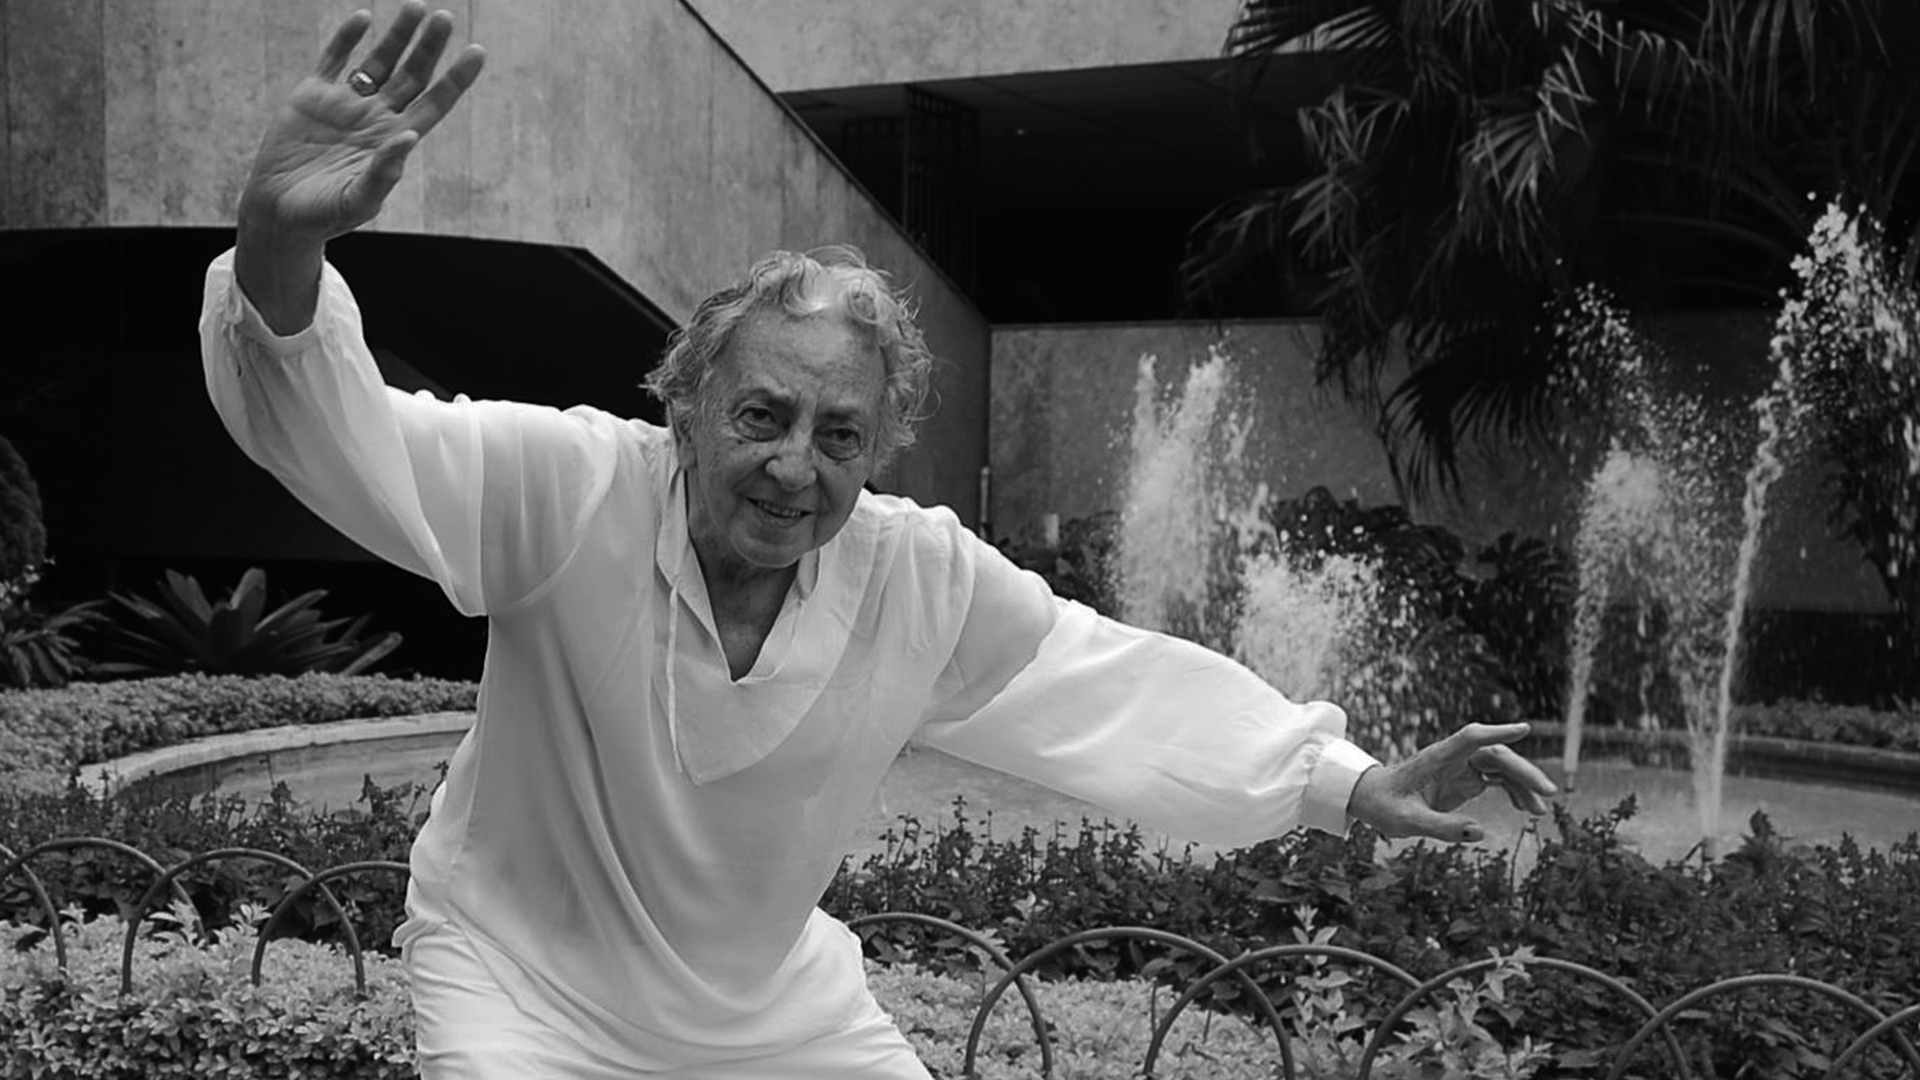
\includegraphics[width=0.45\linewidth]{./figs/rolando}

For Rolando Toro, the inventor and developer of Biodanza, the most important thing was: ``Vivencia, Vivencia, Vivencia''. Thus ``experiencing, experiencing and experiencing''. Indeed, experiencing life through dance, music and movement in group, which enables you to deeply connect with your innerself, each other and the whole. Biodanza lets us feel that life is one and this through a deep and intense bodily experience that is bypassing our mind.

With his system of Biodanza Rolando anticipated against the degeneration of humanity and the human society he observed during the second world war. For Rolando it was clear that the modern men suffers from a disease he called ``society'' that brings them far from their natural state of being, feeling, affection and sympathy, which can trigger anyone to extreme acts of violence and cruelty.

He has developed the system of Biodanza from a nostalgia to love, a system that disseminates love and hope. A system that enables an affective re-education of men whose beauty has been violated by society.
The system of Biodanza thus invites us to take part in a new way of live that is nourished by intense experiences.

Rolando was a passionated scientist and professor in psychology. He developed Biodanza from his own experiences and realised early on that his system has a strong foundation in the life sciences. During his development, he has also been inspired by the founders of modern dance and by primal people who still lay a deep meaning in each movement.

By learning again how to add meaning to each of our movements, we ``re-humanise'' and can find again how to truly live life deeply connected with the beauty of nature surrounding us.

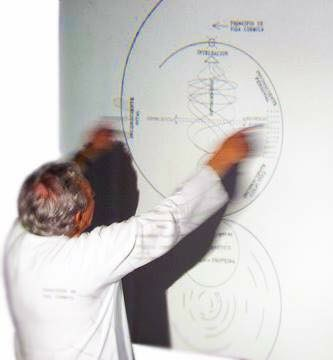
\includegraphics[width=0.45\linewidth]{./figs/rolandoAndModel}

Rolando has laid the foundation of his system during his career as a psychologist/researcher where he discovered the true impact of exercises that stimulate regression and identity, the first axis in his system. As opposed to the conventional mode of action in psychiatry, which has a starting point that is in essence symptomatic, for instance by dosing hormones or neurotransmitters that a patient is lacking, Rolando developed the vision that we could use external stimuli (ecofactors) such as music, movement, touch, caressment, encounters and dance to stimulate our body to produce these substances internally, i.e.~by stimulating our body to tap into its genetic potential, which can promote immense growth.

Growth and learning in Biodanza happens as how children learn: by seeing, imitating, experiencing and repetition, and, this deeply embedded in a stimulating environment with positive reinforcement.

\hypertarget{definition-of-biodanza}{%
\subsection{Definition of Biodanza}\label{definition-of-biodanza}}

Rolando coined the term ``Biodanza'', which is a contraction of ``bios'', the Greek word for ``life'', and, ``danza'' the Italian word for dance. Here, the word dance is used in its original sense of ``natural movement'' that is full of meaning and well-connected with our emotions.

Marcello Mur defines Biodanza in its most simple form as a system of moderate movement and stimulation of sociality.
Rolando Toro as a poetry of encounter. Indeed, all exercises can be seen as a preparation on the encounter with oneself, each other and the whole.

In Rolando's more academic definition Biodanza is a system of human integration, of organic renewal, of affective re-education and of re-learning the original functions of life.

The methodology of Biodanza consists of inducing integrating vivencia through music, singing, movement and encounters in an affective group.

\hypertarget{vivencia}{%
\subsubsection{Vivencia}\label{vivencia}}

The concept of vivencia is key to understand the method of Biodanza.

Vivencia is an intense sensation of living, here and now, with a strong component of total organic sensation that elicits a strong awareness of our bodily existence. It is a manifestation of being that precedes consciousness.
Vivencia are passing experiences, e.g.~vivencia of fullness, of safety, of delight.
The awareness of experiencing vivencia can come instantly or at a later moment and often give rise to deep emotions.

We do not have to try to rationalize our vivencia.
They can be seen as manifestations of our bodily wisdom and spontaneously initiate integration and learning by experience.
They are transformative experiences and are the most important instrument of the method of Biodanza.

\hypertarget{human-integration}{%
\subsubsection{Human Integration}\label{human-integration}}

Through vivencia a strong connection with life is established, which induces the integration with oneself, the human species and the universe.

The integration with oneself restores psychophysical unity, i.e.~the unity of the internal/psychic and external/physical world.

Integration with our fellow humans restores the connection within our species as a biological unity.

Integration with the universe re-unites us with nature and restores our intimate relation with our entire biosphere.
It lets us re-experience the deep connection of ourselves as part of the cosmos.

By restoring this connection to life, we can re-experience life to its very existence, here and now, which promotes a deep conscious awakening.

\hypertarget{organic-renewal}{%
\subsubsection{Organic renewal}\label{organic-renewal}}

Biological systems possess the unique capacity of self-replication and self-organisation. However, stress has a profound impact on cell and tissue maintainance and regeneration.

With Biodanza exercises that aim for regression and integrating transcendence, we slow down our movements, lower our state of control and evoke a deep state of rest. This state is essential to switch on restoration and regeneration, and, reinforces homeostasis, i.e.~our bodies mechanism to maintain its equilibrium despite the oscillations in our environment.

\hypertarget{affective-re-education}{%
\subsubsection{Affective re-education}\label{affective-re-education}}

In Biodanza many exercises stimulate and elicit affection and harmony, which can work through in our daily life by bringing harmony in our relation with ourself, omongst each-other and with our environment.

\hypertarget{re-learning-of-the-original-life-functions}{%
\subsubsection{Re-learning of the original life functions}\label{re-learning-of-the-original-life-functions}}

Biodanza practice also reconnects us with our primal instincts, which are suppressed in our modern society and are often viewed as irrational behavior.
However, our instincts can be viewed as the biological wisdom of our species, which evolved for survival and maintainance of our species. By reconnecting ourselves with our innate impulses, we also restores harmony from within.

\hypertarget{biocentric-principle}{%
\subsection{Biocentric Principle}\label{biocentric-principle}}

The biocentric principle is at the heart of Rolando Torro's system of Biodanza. The biocentric principle considers the universe as the matrix of life i.e., a self-organising structure that is building life. So not only living organisms, but, rather the entire cosmos is viewed as a massive living hologram.

This view invites people to radically rethink their relationship as a human being with the entire biosphere. Indeed, life itself becomes intrinsically sacred, which probes us to put all of life, and thus the entire universe, at the heart of our weltanschauung.

To me, it seems an invitation to gravitate from humanism, with human beings at its center, back to the view of primal cultures where the environment we are living in is not seen as the stage upon which we tread, but as an entity with whom we can communicate and build a deep intimate relationship.

Vivencia is the unique path to experience the Biocentric principle and to genuinely become aware of it. This not through our mind, but, through that deeper knowledge that lies hidden in our inner self, ready to be touched by the intimate vivencial experience.

\hypertarget{model-of-biodanza}{%
\subsection{Model of Biodanza}\label{model-of-biodanza}}

Rolando Toro developed a scheme of his model of Biodanza that covers its foundation in the life sciences and the methodology of Biodanza, which is displayed in Figure \ref{fig:model}.

\begin{figure}

{\centering 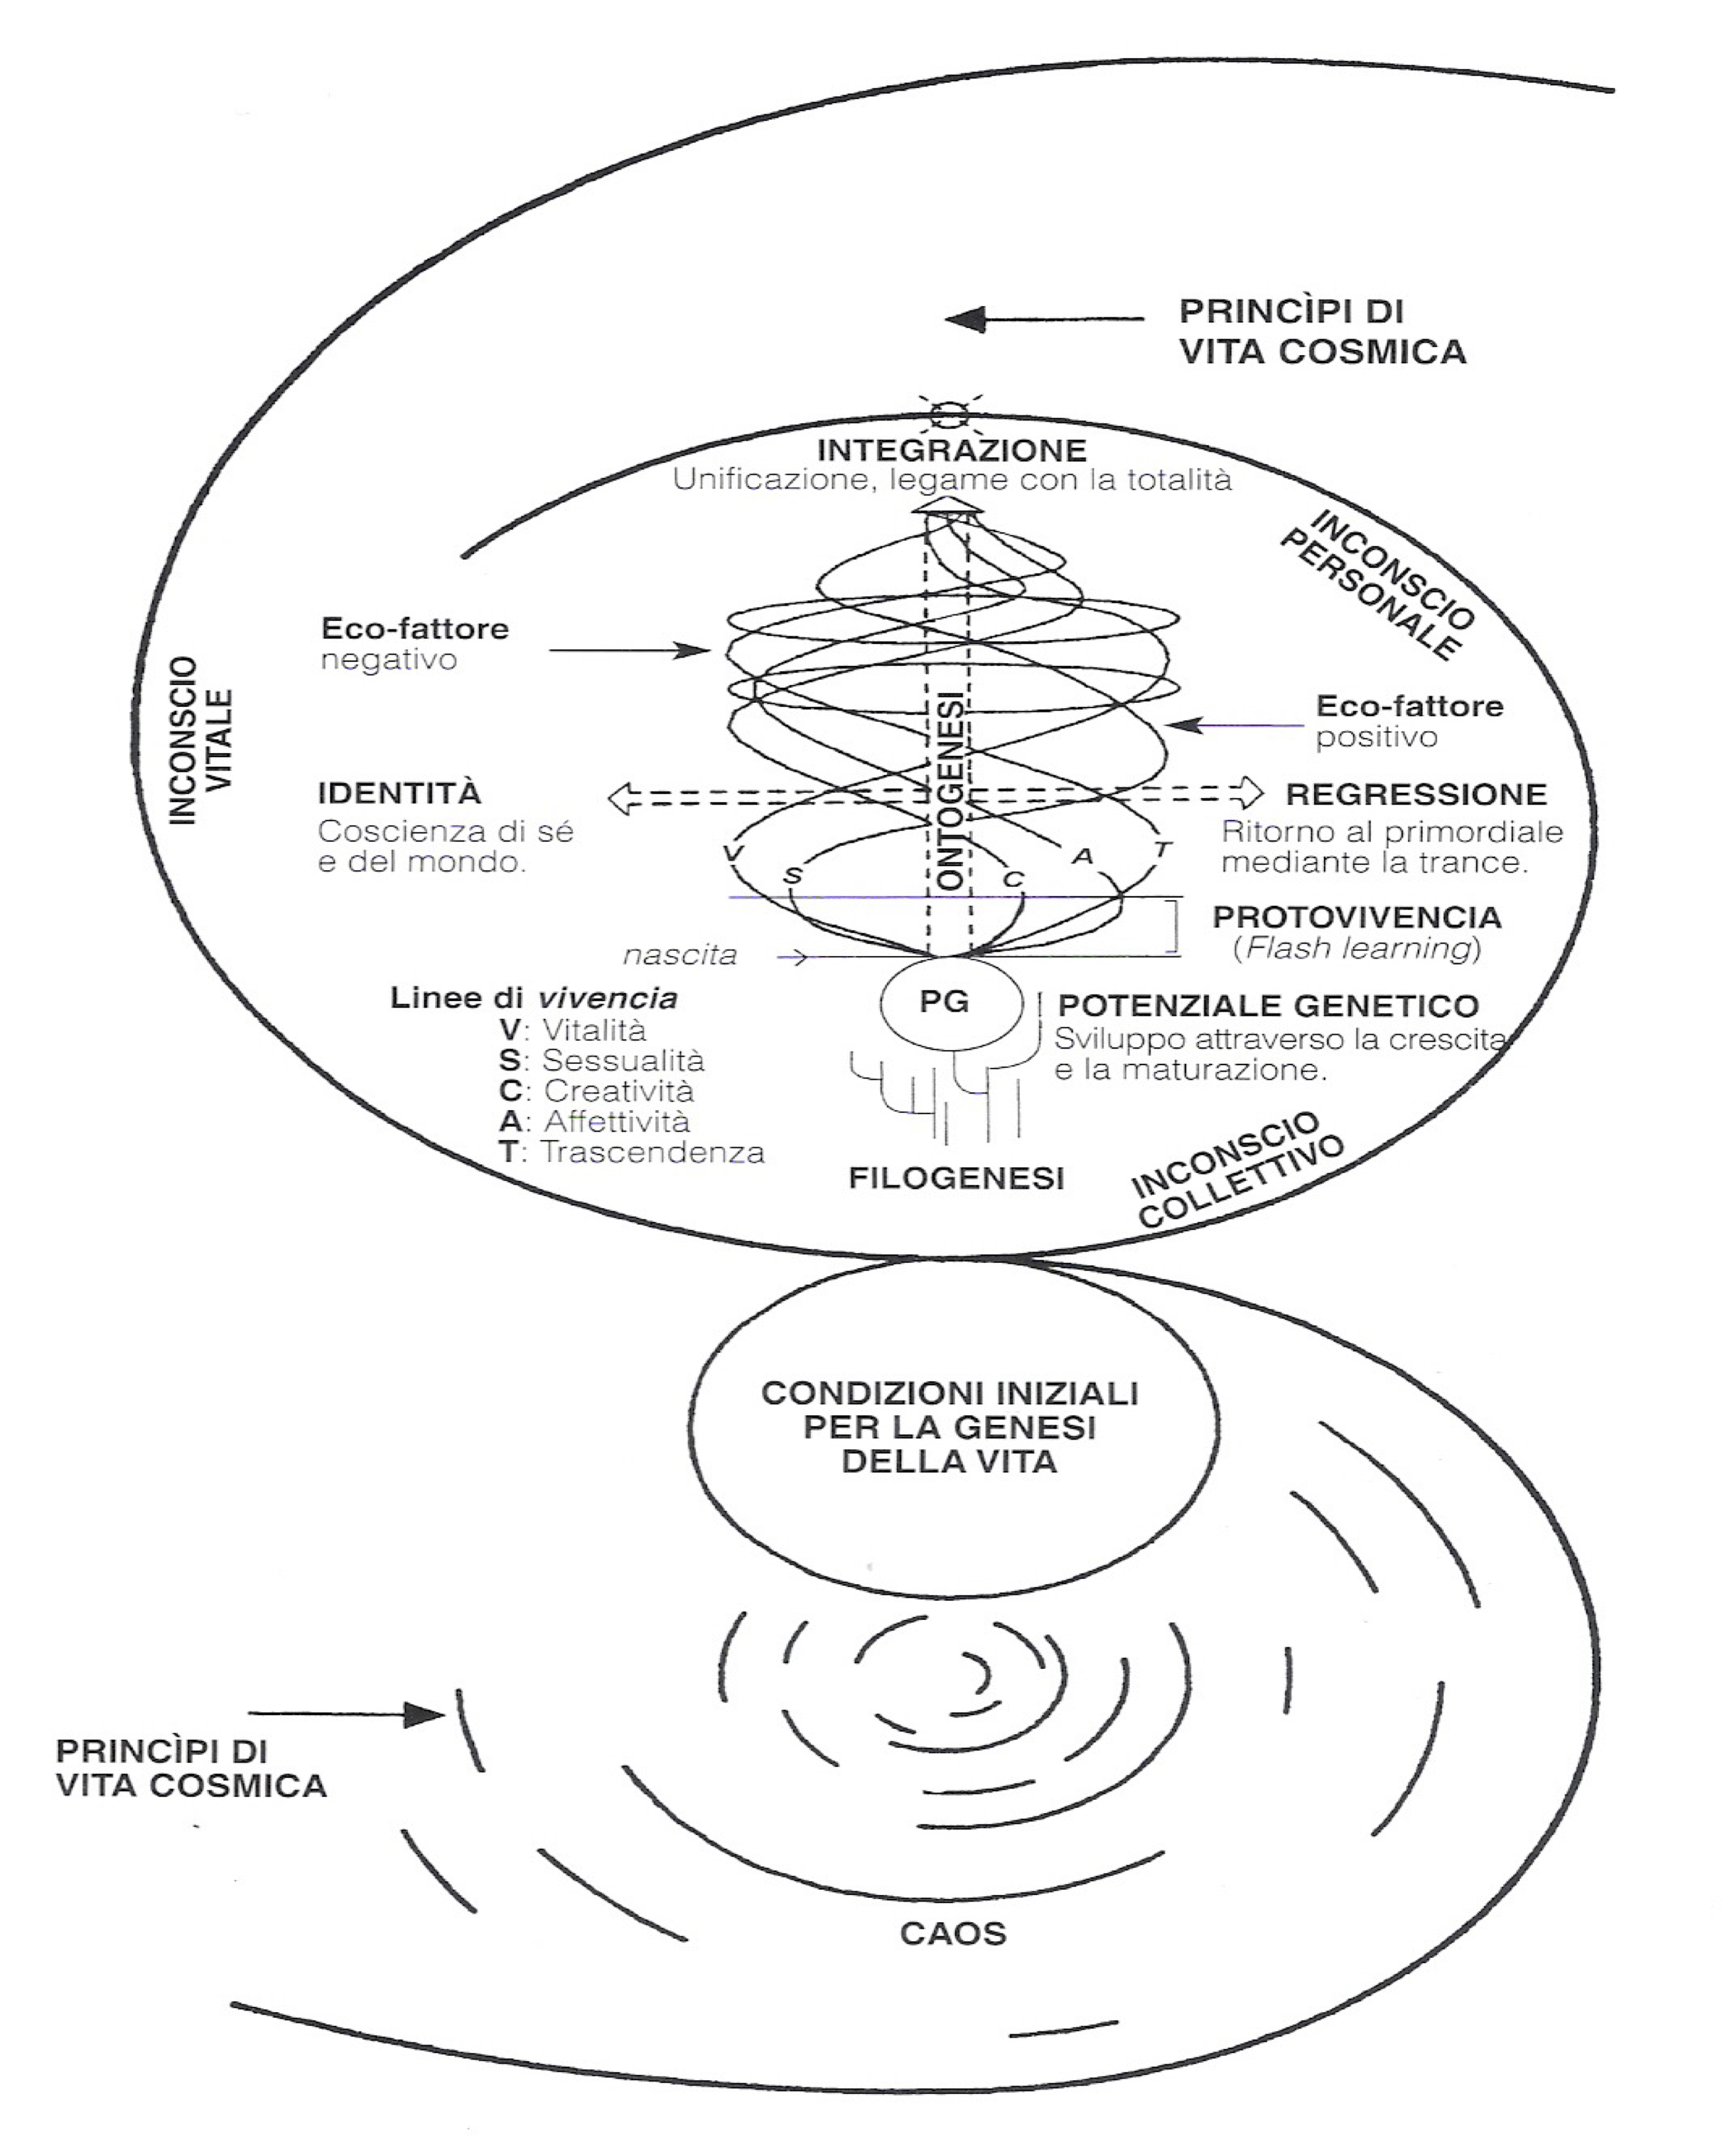
\includegraphics[width=1\linewidth]{./figs/biodanzaModel} 

}

\caption{Model of Biodanza}\label{fig:model}
\end{figure}

In this section I will first briefly introduce the biological aspects in the model of Biodanza, which is the main theme of this monograph, and next I will briefly cover the methodology of Biodanza.

\hypertarget{biological-aspects-of-biodanza}{%
\subsubsection{Biological aspects of biodanza}\label{biological-aspects-of-biodanza}}

The biological aspects of Biodanza can be seen as the skeleton, the vertical axis, in the model of Biodanza see Figure \ref{fig:model}. This axis consists of

\begin{enumerate}
\def\labelenumi{\arabic{enumi}.}
\tightlist
\item
  Principals of cosmic life and genesis of life
\item
  Evolution and phylogenesis
\item
  Genetic potential and ontogenesis
\end{enumerate}

Our cosmos as we know originated out of chaos. It started with a very energy-rich state. It quickly cooled down enough for energy to be converted into mass - the majority in hydrogen and a fraction in more heavy helium nuclei. Due to the gravitational force, matter then started to cluster in nebula and eventually in stars.

In the stars all elements have been formed by nuclear fusion and with each supernova, explosion of a star at the end of its life, these elements/atoms are projected into space.

In space these atoms further reacted and formed more complex molecules that eventually gave rise to precursors of the biological building blocks of life.

In a remote corner of our milky way, an average galaxy, on an average planet, our earth, there originated unique conditions that made abiogenis or the \emph{genesis of life} possible.
This was initiated by a chemical evolutionary process that gave rise to molecules with increasing complexity ultimately leading to chemistry that enabled self-replication and self-organisation and to the four essential bio-molecules of which all life is built:

\begin{itemize}
\tightlist
\item
  Lipids that enable the formation of membranes that are separating the inside of the cell from the outer world,
\item
  Carbohydrates or sugars that are used as energy sink/resource and as a backbone of many bio-molecules,
\item
  Proteins, the workhorses in our cells that facilitate the majority of chemical reactions in our cells, and
\item
  Nucleic acids, DNA and RNA, that are used to store and use our genome, the set of genes, we inherited from our parents.
\end{itemize}

Once the first living cells emerged, they started to evolve and through evolution, they gave rise to all other living beings. This process is also referred to as phylogenesis.

We, humans, are a leaf on a small branch of the tree of life. Each of us with our own genetic potential. Through the course of our life, we develop from a fertilized egg cell to embryo, a child upto a full grown adult until we eventually die. During this process, which is also referred to as ontogenesis, the way how we use our genes is changed.

Indeed, at the conception we inherit the structure of our cells from our biological mothers' egg cell and our genome from our biological mother and father. At first this egg cell has access to all genes. But, as the cell divides into a clump of cells that starts to differentiate in different tissues, the more specialized cells have only access to a restricted set of genes that are essential for their function. This happens through small molecules that interact with our DNA and can switch genes on or off.
The study of how our behavior, development and environment can cause changes that affect the way your genes work is also referred to as epigenetics.

Epigenetic changes are passed in cell devision to the two new cells that are formed, which makes a liver cell to remain a liver cell and a brain cell to remain a brain cell upon cell division.

Also, external stimuli and eco-factors can induce epigenetic changes and can thus effectively shape how we use our genetic potential. This is exactly what we aim for with the methodology of Biodanza, which lies at the heart of the model of Biodanza.

\hypertarget{methodology-of-biodanza}{%
\subsubsection{Methodology of Biodanza}\label{methodology-of-biodanza}}

With Biodanza practice, we can effectively shape how our genetic potential is used. Indeed, when we experience a deep vivencia, this is accompanied by intense bodily experiences. So a Biodanza session induces physiological changes, and can thus effectively trigger the production of hormones, neurotransmitters and proteins, which originate from the expression of specific genes in our body and brain.

People who practice Biodanza for a longer period also experience that it can have a deep impact on their life and their social interactions, which is the result of rewiring in the brain.

So we can see the methodology of Biodanza as an effective tool to interact with and to impact on our body, the expression of our genes and thus how we use our genetic potential.

The methodology of Biodanza is the central part in the model of Biodanza see Figure \ref{fig:model}, which I view as the meat that is added to the skeleton of life.

\hypertarget{horizontal-axis-identity-vs-regression}{%
\paragraph{Horizontal axis: Identity vs Regression}\label{horizontal-axis-identity-vs-regression}}

Rolando has laid the foundation of his system during his career as a psychologist/researcher where he discovered the true impact of exercises that stimulate regression and identity, the horizontal axis in his system.

Each Biodanza session starts with exercises that make participants aware of their body and their identity through rythmic activating exercises.
Then we make the bridge to more deepening exercises where we slow down our movements to lower our state of control, which evoke trancendence and integration, and thus the connection to oneself, our human species and the whole.

\hypertarget{vertical-axis-five-lines-of-biodanza}{%
\paragraph{Vertical axis: five lines of Biodanza}\label{vertical-axis-five-lines-of-biodanza}}

Rolando structured our genetic potential in five lines: vitality, affection, creativity, sexuality and transcendence.
In a biodanza session we typically work in two or more of these lines.

In the model the five lines are spiraling around the vertical axis of ontogenesis. Indeed, in a Biodanza session we bomb the participants with ecofactors that stimulate these five lines and that can have long-lasting effects on a genomic and physiological level.

We already get in touch with these five lines very early on in our lifes, which Rolando referred to as protovivicencia. Indeed, as a baby we experience these protovivencia, e.g.~through attention, food, love, care, caressment and harmony in our environment.

During a Biodanza session we let (a subset of) the five lines pulsate by a sequence of exercises that first focus on identity and then on regression.
Exercises that strengten identity let practitioners become more aware of themselves, the world around them and how they stand in that world. Regression on the other hand stimulates the identity to dissolve, promoting a connection with ones inner self, each-other, our species and our entire biosphere.

\hypertarget{unconsciousness}{%
\paragraph{Unconsciousness}\label{unconsciousness}}

In the periphery of methodology of Biodanza in the Model, see Figure \ref{fig:model}, we find the personal unconsciousness, collective unconsciousness and vital unconsciousness.
Which is a resonance with ideas and information on ourself, our primal instincts and archetypes, and the information that pulsates in the matrix of life, respectively.

Indeed, when a father caresses his baby, he connects with
his personal unconsciousness through the bound he experiences with his child, with the Demeter or mother archetype in his collective unconsciousness, and, with his vital unconsciousness through the physiological response he experiences through the proteins, hormones and neurotransmitters that are expressed in his cells.

So many of our actions are steered by our unconsciousness.
Through Biodanza exercises on regression we can deeply connect with these three types of unconsciousness which stimulates a deep sense of connectedness with oneself, each-other and the whole.

When practicing Biodanza on a long term we stimulate our genetic potential, integration and connectedness with ourself, our species, all of life, the whole, for which Rolando uses the metaphor ``the cosmic human''.

\hypertarget{aims-of-this-monograph}{%
\subsection{Aims of this monograph}\label{aims-of-this-monograph}}

This monograph focuses on the Biological aspects of Biodanza and originates from the module on Biological aspects of Biodanza for which I have given the theory in the school of Antwerp.

In particular, I will try to place all concepts that appear in the official learning material of the Scuolatoro, the Motherschool of Biodanza, in the context of the Model of Biodanza in a humble attempt to provide more insight for Biodanza practitioners and facilitators without a formal scientific background.

This attempt consists of five parts:

\begin{enumerate}
\def\labelenumi{\arabic{enumi}.}
\item
  What is Life, which gives a basic foundation and introduces important biological concepts that might provide a deeper insight in

  \begin{itemize}
  \tightlist
  \item
    the biocentric principle and
  \item
    vital unconciousness
  \end{itemize}
\item
  Principles of Cosmic Life and the Genesis of Life, which I will try to introduce in a short narrative on the history of the universe up to the origin of life.
\item
  Evolution and Phylogenesis, which tells a brief story on the history of life and how life evolved.
\item
  Ontogenesis, which tries to shed some light on how our cells evolve from our origin as a fertilized egg cell up to our adult stage until we eventually die.
\item
  Ontogenesis and Biodanza, a short view on how the method of Biodanza might impact ontogenesis in our path towards integration
\end{enumerate}

\end{document}
